\documentclass[11pt]{article}

\setlength\parindent{0pt}
\setlength{\parskip}{.25\baselineskip}

\usepackage{hyperref}
\usepackage{amsmath,amsfonts,amssymb,bbm}
\usepackage{todonotes}
\usepackage{subcaption}

\DeclareMathOperator{\Tr}{Tr}
\newcommand{\R}{\mathbbm{R}}
\newcommand{\mba}{\mathbf{a}}
\newcommand{\mbb}{\mathbf{b}}
\newcommand{\mbx}{\mathbf{x}}
\newcommand{\mbxt}{\tilde{\mathbf{x}}}
\newcommand{\Sigmat}{\tilde{\Sigma}}
\newcommand{\mbz}{\mathbf{z}}
\newcommand{\mbw}{\mathbf{w}}
\newcommand{\mcN}{\mathcal{N}}
\newcommand{\mcP}{\mathcal{P}}
\newcommand{\eps}{\epsilon}
\newcommand{\trans}{\intercal}
\newcommand{\Ut}{\tilde{U}}
\DeclareMathOperator*{\argmax}{arg\,max}

\title{A Probabilistic Model for Astronomical Source Discovery and Separation}
\author{Andrew Miller, Albert Wu, Brenton Partridge, Ryan Adams, ...}
\date{\today}

%% DOC START
\begin{document}
\maketitle
\tableofcontents
\newpage

\section{Introduction}

The goal of this project is to develop reliable inference techniques to simultaneously discover and characterize properties of distant stars and galaxies from a massive database of photometric imagery.  

We define notation: 
\begin{itemize} \itemsep 0pt
\item $s \in \{1, \dots, S\}$ will index unique sources (stars or galaxies)
\item $n \in \{1, \dots, N\}$ will index unique images
\item $\beta_n \in \{r, \dots, z\}$ will stand for the band of image $n$
\end{itemize}

We note that the number of sources, $S$, is unknown a priori and modeled as a random variable.  For each source, we define the following \emph{intrinsic} properties, which are the estimands of interest: 
\begin{align*}
  c_s &= \text{ class of source } \in \{ \text{star}, \text{galaxy}, \text{quasar} \} \\
  u_s &= (u_{s,ra}, u_{s,dec}) = \text{right ascension and declination of source $s$} 
\end{align*}

For stars (point sources), we are interested in estimating the following properties 
\begin{align*}
  t_s &= \text{temperature of source $s$ (kelvin)} \\
  d_s &= \text{distance to source $s$ (meters)} \\
  \ell_s &= \text{luminosity of source $s$ (Joules/second)} 
\end{align*}

For galaxies, we define the following intrinsic properties 
\begin{align*}
  \theta &= \text{mixing proportion between De Vaucouleurs and Exponential profiles} \\
  b_s    &= (b_{s,u}, \dots, b_{s,z}) \text{ band-wise brightnesses } \\
  R_s    &= \text{matrix encoding shape and rotation} \\
  z_s    &= \text{red shift}
\end{align*}

For quasars, we want to characterize the following properties 
\begin{align*}
  z_s &= \text{red shift} \\
  b_s &= (b_{s,u}, \dots, b_{s, z}) \text{band-wise brightnesses?}
\end{align*}

In all cases, source properties will be inferred by the intensity (amount) and color (distribution across bands) of photons captured in imagery.  An example of such photometric observations are depicted in Figure~\ref{fig:bands}.  




This paper describes a probabilistic model-based approach to inferring these quantities of interest.  We treat the observed pixel values as random variables, and describe a (stochastic) forward generating procedure based on the properties of these sources (the likelihood), as well as an a priori distribution over the properties themselves (the prior), and use Bayesian inference and Markov Chain Monte Carlo techniques to draw simulations from the posterior.  To understand the likelihood, we first outline the physical motivation underlying our model.  

\begin{figure}[t!]
\begin{center}
\begin{subfigure}[a]{.3\textwidth}
  \includegraphics[width=\textwidth]{{"imgs/data/nelec-u"}}
  \caption{u band}
\end{subfigure}
\begin{subfigure}[a]{.3\textwidth}
  \includegraphics[width=\textwidth]{{"imgs/data/nelec-g"}}
  \caption{g band}
\end{subfigure}
\begin{subfigure}[a]{.3\textwidth}
  \includegraphics[width=\textwidth]{{"imgs/data/nelec-r"}}
  \caption{r band}
\end{subfigure}
\begin{subfigure}[a]{.3\textwidth}
  \includegraphics[width=\textwidth]{{"imgs/data/nelec-i"}}
  \caption{i band}
\end{subfigure}
\begin{subfigure}[a]{.3\textwidth}
  \includegraphics[width=\textwidth]{{"imgs/data/nelec-z"}}
  \caption{z band}
\end{subfigure}
\end{center}
\caption{SDSS photon count images.  Each image corresponds to one band These five images have been aligned - each corresponding to the same viewing frame, among 5 bands. Five sources are visible - their intensity/number of photon observations are a function of their temperature, luminosity, and distance to earth.}
\label{fig:bands}
\end{figure}


\section{Modeling stars}
The random variable that gives rise to our likelihood and motivates probabilistic inference in this problem is the number of photons detected by an instrument with a lens of a fixed area over a fixed exposure duration.  According to our idealized model, this random variable is Poisson distributed conditioned on the intrinsic properties of a source.  To describe our observations, we need to outline the procedure by which the band-specific flux images are generated.  

To compute how many photo-electrons we expect to be captured by a lens of size $A$ over exposure duration $\Delta$, we must compute the number of photons that will eventually be intercepted by the instrument as a function of the source's distance, luminosity, and temperature.  Geometrically, we can view the source as a single point in space at a distance $d_s$, which radiates energy uniformly outward, such that the level sets of equal radiation form a sphere.  We can think of the area of the lens of the instrument as some fraction of the total surface area of this sphere, which is, roughly
\begin{align}
  \frac{A}{4\pi d_s^2} &= \text{ proportion of surface area detected }
\end{align}
If a source is emitting $\ell_s$ Joules per second, the amount of energy that actually is detected by the instrument dissipates as the proportion of surface area decreases, which falls off $\frac{1}{d_s^2}$ as a function of distance (e.g. if we had a `lens' that formed a perfect sphere around the black body, we could effectively measure all $\ell_s \Delta$ Joules for an exposure of length $\Delta$).  

To obtain the total number photo-electrons we expect to detect in band $\beta_n$, we need to compute how much of a black body's energy is distributed within the spectrum recorded by $\beta_n$ \emph{and} account for how our instrument filters $\beta_n$ over a chunk of the energy spectrum (non-uniformly, see Figure~\ref{fig:sensitivity}).

Intuitively, we can do this by computing the photon flux as a function of source temperature and wavelength, and then integrate this value times the sensitivity curve to obtain the total amount of energy we expect the black body to emit per unit area per unit time.  
\begin{align}
  \text{\# P-E detectable in band $\beta_n$} &= I_{\beta_n}(t_s) \cdot \ell_s \frac{A \Delta}{4\pi d_s^2}  
  \label{eq:brightness}
\end{align}
which reads the number of photo-electrons detectable by our instrument in band $\beta_n$ due to a single source $s$ is simply the number of photons we expect to see per unit energy that a source at temperature $t_s$ emits in band $\beta_n$ (modulated by our instrument filter $S_\lambda$) times the total luminosity of the source (energy emitted per second) times the fraction of the sphere at distance $d_s$ we can actually detect times the duration of exposure.  The simple geometric approximation for $\frac{ A \Delta }{ 4 \pi d_s^2 }$ will suffice for that term.  To compute $I_{\beta_n}(t_s)$, we must compute the spectral energy density of an idealized black body, for which we appeal to Planck's law. 

\begin{figure}[t!]
\begin{align*}
  B(t, \lambda) &= \frac{2 h c^2}{\lambda^5} \frac{1}{ e^{\frac{hc}{\lambda k_B t}} - 1} \text{ (Planck's law) } \\
  \int B(t, \lambda) &= P(t) = \frac{\sigma}{\pi} t^4  \text{ (Stefan-Boltzmann) }\\
  E(\lambda) &= \frac{hc}{\lambda} \\
  S(\lambda) &= \text{ instrument sensitivity - lookup table } \\
  A &= \text{ lens area (meters$^2$) } \\
  \Delta  &= \text{ exposure duration (seconds) } \\
  c &= \text{ speed of light (meters / second) } \\
  h &= \text{ Planck constant } \\
  k &= \text{ Boltzmann constant } \\
  \sigma &= \text{ Stefan-Boltzmann constant } 
\end{align*}
\caption{Relevant physical relationships and constants}
\end{figure}

\subsection{Planck's Law}
Our goal is characterize the distribution of energy radiated by an idealized black body as a function of definite temperature and wavelength, which is the relationship described by Planck's law, which tells us that the spectral radiance is given by
\begin{align}
  B(t, \lambda) &= \frac{2 h c^2}{\lambda^5} \frac{1}{ e^{\frac{hc}{\lambda k_B t}} - 1}
\end{align}
which is in units of Watts per steradian per meter$^2$ per wavelength unit.  Intuitively, this describes the distribution of energy over the spectrum.  

The total radiance across all wavelengths per square meter per steradian is given by the Stefan-Boltzmann law, which is easily computed as 
\begin{align}
  P(t) = \frac{\sigma}{\pi} t^4 \text{  in J / (s $\cdot$ m$^2$ $\cdot$ str) } 
\end{align}
which is obtainable if you integrate the relationship in Planck's law over wavelength.  Simply dividing the two relationships gives you the energy density, or the \emph{distribution} of energy over the spectrum you expect the black body to exhibit.  We are interested in actual photon counts, so we will want to include the relationship between energy and photons as wavelength varies, given by 
\begin{align}
  E(\lambda) &= \frac{h c}{\lambda} \text{ in J / photon }
\end{align}
Now we must consider the sensitivity of our instrument with respect to wavelength, which allows us to compute our per-wavelength photo-electron fluxes (counts per unit time) as 
\begin{align}
  F(t, \lambda) &= \frac{B(t, \lambda)}{P(t)} \frac{S_{\beta_n}(\lambda)}{E(\lambda)} 
\end{align}
where $S_{\beta_n}(\lambda)$ is the sensitivity filter for band $\beta_n$, which is a function of $\lambda$ with range in the unit interval.  The above value is the number of photons detectable by our sensor per unit wavelength.  

Finally, integrating over wavelength (which will be approximated numerically) will yield the expected number of photo-electrons detected by our instrument in a given band from a source 
\begin{align}
  I_{\beta_n}(t_s) &= \int_{\beta_n} \frac{B(t_s, \lambda)}{P(t_s)} \frac{S_{\beta_n}(\lambda)}{ E(\lambda)} d\lambda
  \label{eq:photojoules}
\end{align}
which gives us the number of photo-electrons per Joule we expect to see from the source in band $\beta_n$.  This is \emph{almost} the random variable we actually observe.  These photo-electrons are then spread out by the instrument according to a calibrated point-spread function (PSF).  The PSF model is known, and will finally relate the observed pixel values to the source's intrinsic properties. 

We can express the numerical integration as a dot product
\begin{align}
  \hat I_{\beta_n}(t_s) &= \mathbf{f}_{t_s}^\trans \mathbf{h_{\beta_n}} \\
  \mathbf{f}_{t_s}     &= (B(t_s, \lambda_1)/P(t_s), \dots, B(t_s, \lambda_L)/P(t_s)) \\ 
  \mathbf{h}_{\beta_n} &= (S_{\beta_n}(\lambda_1)d\lambda / E(\lambda_1), \dots, S_{\beta_n}(\lambda_L)d\lambda / E_{\lambda_L}) 
\end{align}
where $\mathbf{f}_{t_s}$ is the vector approximation to the spectral density of a black body at temperature $t_s$, and $\mathbf{h}_{\beta_n}$ is the vector approximation of the 
which will be a convenient representation when we differentiate the likelihood with respect to $t_s$.  

\subsection{Putting it together}
We can now compute the number of photons from a source as observed in an image by combining Equation~\ref{eq:brightness} with Equation~\ref{eq:photojoules} to yield
\begin{align}\label{eq:photosource}
  c(t_s, d_s, \ell_s, \beta_n) &= 
    \underbrace{I_{\beta_n}(t_s, S_\lambda)}_{
      \substack{ \text{\# photons detectable} \\
                 \text{in band $\beta_n$ from a } \\
                 \text{source at temp} \\
                 \text{$t_s$ per Joule}}} \cdot 
    \underbrace{ \ell_s }_{
      \substack{ \text{ Joules/sec } \\
                 \text{ radiated by} \\
                 \text{ source $s$ } }} \cdot
    \underbrace{ \frac{A}{4\pi d_s^2} }_{
      \substack{ \text{ proportion of } \\
                 \text{ sphere measurable } \\
                 \text{ by instrument }}} \cdot
    \underbrace{ \Delta }_{
      \substack{ \text{ exposure } \\
                 \text{ duration (s) } } }
\end{align}
giving us the expected number of photons that source $s$ contributes to image $n$.  

\begin{figure}[t!]
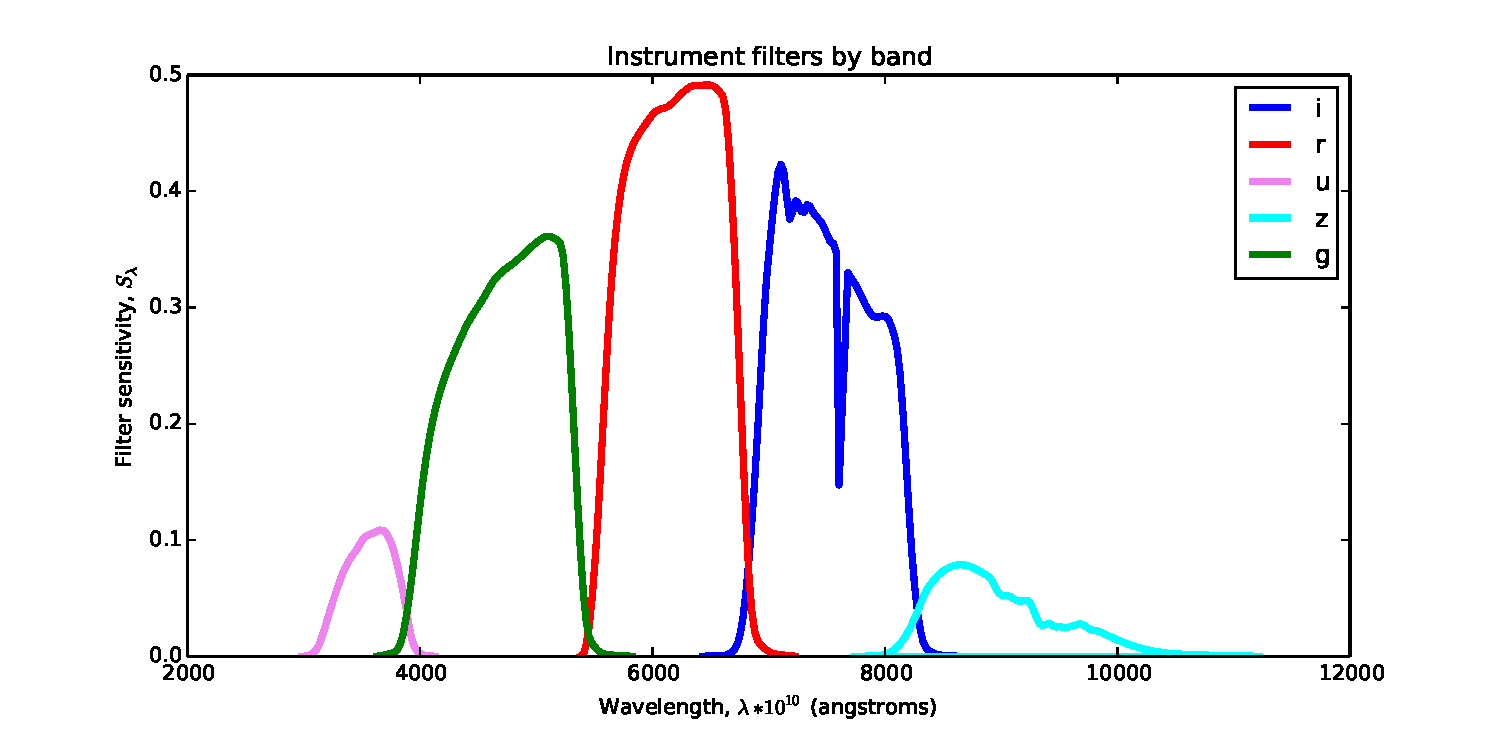
\includegraphics[width=\textwidth]{imgs/filter_sensitivity.pdf}
\caption{Instrument filter sensitivity curves in each band.  The amount of energy (i.e. number of photo-electrons detected) are are not collected uniformly across the range of wavelengths detected in each band - they are scaled according to these curves.  The total count for each band will be the integral of number of photo-electrons detected in each wavelength (energy level), scaled by these curves. }
\label{fig:sensitivity}
\end{figure}

\subsection{From Sources to Pixel Observations}
An image $n$ corresponds to measurements in one band, $\beta_n$, and consists of pixels locations denoted by $m = (w,h)$.  The total number of photons we expect to observe in image $n$ is simply the sum of the contribution we expect to see from each source, described above.  However, this total number is distributed about the pixels of the image according to the image's point spread function (PSF), due to atmospheric turbulence.  For image $n$ (with only point source contributions) and pixel $m = (w,h)$, where $m \in \mathcal{P}_n$ denotes a pixel in the set of pixels associated with image $n$, the distribution over photon count is modeled
\begin{align}
  x_{n,m} | \{(u_s, t_s, \ell_s, d_s)\}_{s=1}^S &\sim \textrm{Poisson}( \epsilon_n + \sum_{s=1}^S F_{n,m,s} ) \\
  F_{n,m,s} 
    &= c(t_s, d_s, \ell_s, \beta_n) f_s(m)  \\
    &= \underbrace{\mathbf{f}_{t_s}^\trans \mathbf{h_{\beta_n}}}_{I(t_s, \beta_n)} \cdot 
       \underbrace{\frac{\ell_s}{4 \pi d_s^2}}_{b_s} \cdot
       \underbrace{A \Delta}_{lens} \cdot 
       \underbrace{f_s(m,n)}_{psf} \\
 \epsilon_n &\sim \textrm{Gamma}(\alpha, \beta) \\
  f_s(m)  &= \sum_{k=1}^3 w_{n,k} \phi(m; v_{n,s} + \mu_{n,k}, \Sigma_{n,k}) \\
  v_{n,s} &= \Upsilon_n(u_s - \phi_n) + \rho_n
\end{align}
where 
\begin{itemize}
  \item $w_{n,k}, \mu_{n,k}, \Sigma_{n,k}$ for $k=1,2,3$ parameterizes image $n$'s point spread function (PSF) in pixel coordinates
  \item $f_s(m)$ is the amount of the source that is assigned to pixel $m$ (the PSF itself)
  \item $\epsilon_n$ acts as a bias term, explaining counts unexplained by sources in image $n$ 
  \item $v_{n,s}$ is the location of the source in pixel coordinates, an image-specific linear transformation of $u_s$. 
\end{itemize}
Due to an identifiability issue, we can only infer the ratio of $\ell_s$ and $d_s^2$, which we instead parameterize it's \emph{apparent brightness} (measured in Joules per meter$^2$ second)
\begin{align}
  b_s \equiv \frac{\ell_s}{4 \pi d_s^2}
\end{align}

We can write the likelihood as 
\begin{align}
   L(\{u_s, t_s, b_s\}_{s=1}^S)
     &= \prod_{n=1}^N \prod_{m \in \mathcal{P}_n} p_{pois}(x_{n,m} ; F_{n,m}) \\
     &= \prod_{n,m} \frac{ F_{n,m}^{x_{n,m}}}{x_{n,m}!} e^{-F_{n,m}}
\end{align}
where $\mathcal{P}_n$ denotes the set of pixels in image $n$.  

and the log likelihood, over all images, as 
\begin{align}
  \log L(\{u_s, t_s, b_s\}_{s=1}^S) 
    &= \underbrace{\sum_{n=1}^N}_{\text{images}}
       \underbrace{\sum_{m \in \mathcal{P}_n}}_{\text{pixels in $n$}}
       \log p_{pois}(x_{n,m}; F_{n,m}) \\
    &= \sum_{n,m} x_{n,m} \log F_{n,m} - F_{n,m} + const.
\end{align}
One problematic aspect of the likelihood is the $\log F_{n,m}$ term, which is difficult to directly optimize and compute with multiple cores.  We can simplify this by using a natural latent variable representation of additive Poisson intensity functions.  

\section{Galaxies}
This section will describe the likelihood of a source conditioned on it being of class $c_s = 1$ (Galaxies).  Galaxies differ from point sources in that photometric observations have spatial extent that is not solely due to the point spread function.  There is both a shape and function that describes the spatial distribution of light due to the galactic source as observed from Earth.  This shape is then further convolved with the point spread function in a similar way to stars.  

The three appearance elements of a galaxy in our model are due to 
\begin{itemize}
\item Galactic profile (De Vaucouleurs vs Exponential profiles)
\item Rotation and scaling 
\item Point spread function 
\item Total intensity and color distribution 
\end{itemize}

This section outlines a probabilistic model to describe how those four components generate the photometric Poisson distributed observations. Firstly, we employ the use of a mixture of Gaussians method of \todo{cite Hogg and Lang} to describe the galaxy's profile, rotation and scaling, and straightforward convolution with the point spread function to describe the spatial observation of galaxies.  The total intensity and color distribution are then generated from prior distribution (left generic for now).

\todo{At the moment there is no red-shift inference for Galaxies}

The galactic profiles are simply isotropic, concentric mixtures of Gaussians with known parameters.  For a pixel $m$, spatial distribution of photons from a source centered on pixel $(0,0)$ for De Vaucouleurs and Exponential would be
\begin{align}
  p_{dev}(m) &= \sum_{k=1}^{K_{dev}} w_{dev, k} \mathcal{N}\left(m | 0, \sigma^2_{dev, k} I \right) \\
  p_{exp}(m) &= \sum_{k=1}^{K_{exp}} w_{exp, k} \mathcal{N}\left(m | 0, \sigma^2_{exp, k} I \right)
\end{align}

The rotation matrix $R_s$ defines a covariance for each of the mixtures, $\sigma_{\cdot, k} R_s R_s^\trans$. 

Denoting $\theta_{s,1} \equiv \theta_{s}$ and $\theta_{s,2} \equiv 1-\theta_{s}$, and $K_1 \equiv K_{dev}$, $K_2 \equiv K_{exp}$ for convenience, the generative model for an image patch depicting only galaxies is 
\begin{align}
  \theta_s &\sim p_\theta \\
  b_s      &\sim F_{gal-bright} \\
  R_s      &\sim F_{R} \\
  x_{n,m} | \{ \theta_s, b_s,...\}_{s=1}^S &\sim \textrm{Poisson}\left( \epsilon_n + \sum_{s=1}^S F_{n,m,s} \right) \\
  F_{n,m,s} &= b_{s, \beta_n} f_{n,m,s} \\
  f_{n,m,s} 
    &= \sum_{k=1}^{K_{psf}} w^{(ps)}_{n,k} 
       \sum_{i=1}^2 \theta_{s,i} 
       \sum_{j=1}^{K_i} w_{i, j} \\
       & \mathcal{N} \left(m | u_s + \mu^{(psf)}_{n,k}, \Sigma^{(psf)}_{n,k} + \sigma_{i,j} R_s R_s^\trans \right)
\end{align}

The giant mixture of Gaussians is the result of convolving the image's PSF (mixture of 3 Gaussians) with the mixture of both profiles (essentially a mixture of $K_1 + K_2$ Gaussians), yielding a mixture of $3(K_1 + K_2)$ Gaussians.  \todo{I think it's $3 \cdot (8 + 8)$}
 
Note that the PSF mixture weights, means and covariances are image (and therefore band) specific. 


\section{Inference}

\subsection{Latent Variable Representation}
A convenient property of Poisson random variables with additive intensity functions is that they can be viewed as independent Poisson random variables that have been summed, that is
\begin{align}
  X &\sim \textrm{Poisson}(\lambda_1 + \lambda_2 + \dots + \lambda_S) \\
  X_s &\sim \textrm{Poisson}(\lambda_s) \text{ independent for } s = 1, \dots, S \\
  \implies
  X &\sim \sum_{s=1}^S X_s
\end{align}
So we can represent a Poisson random variable, $X$, as the sum of $S$ Poisson random variables, each corresponding to a piece of the original intensity function.  This is a convenient representation if those additive pieces of the intensity function have a useful interpretation, such as photon contribution from individual sources.  Given the sum of $S$ Poisson random variables, the individual components, $X_1, \dots, X_S$ have a multinomial distribution 
\begin{align}
  X_1, \dots, X_s | X=x &\sim \textrm{Mult}\left(n=x, p= \frac{\lambda_1}{\sum \lambda_s}, \dots, \frac{\lambda_S}{\sum \lambda_s} \right) 
\end{align}

We can adopt this latent variable representation in the generative image model.  For each pixel we introduce the latent variables
\begin{align}
 Z_{n,m} = (Z_{n,m,0}, Z_{n,m,1}, \dots, Z_{n,m,S})
\end{align}
where each component can be interpreted as the number of photons observed in pixel $m$ of image $n$ due to source $s$, and $Z_{n,m,0}$ is reserved for the background photons.  

Conditioned on $\{Z_{n,m}\}$, we can re-write the likelihood as 
\begin{align}
  L(\{u_s, t_s, b_s\}_{s=1}^S; \{z\})
     &= \prod_{n=1}^N \prod_{m \in \mathcal{P}_n} \prod_{s=0}^S  p_{pois}(z_{n,m,s} ; F_{n,m, s}) 
\end{align}
where we define $F_{n,m,0} \equiv \epsilon_n$.  For an image $n$ and a source $s$, we can gather all photons assigned to that source add them
\begin{align}
  z_{n,m,s} &\sim \textrm{Pois}(F_{n,m,s}) \\
  \sum_{m} z_{n,m,s} &\sim \textrm{Pois}\left( \sum_{m} F_{n,m,s} \right) \\
    &\sim \begin{cases}
         \textrm{Pois}( c(t_s, d_s, \ell_s, \beta_n) ) & \text{ if } s > 0  \\
         \textrm{Pois}( M_n \epsilon_n ) & \text{ if } s = 0 
       \end{cases}
\end{align}
which is due to the fact that the PSF is a density, so it sums to one (note that this assumes that image $n$ contains the entire support of the PSF, which will eventually be approximated).  

Conditioning on $Z$ allows us to consider the sources independently.  This will prove important when fitting source-specific parameters.  We will either sample (or impute) $Z_{n,m,s}$ for each pixel, and then sample (or maximize) over $u_s, t_s, b_s$ independently across sources.  

\subsection{Initialization with EM}
The goal of this section is derive a routine to find the maximum likelihood values for $\{ u_s, t_s, b_s \}_{s=1}^N$ (and $\{ \epsilon_n \}_{n=1}^N$ for a fixed number of sources $S$.  This will give us an initialization for star parameters (or allow us to sample over a conditional likelihood).  With a fixed number of sources, $S$, the latent variable formulation admits a simple and parallelize-able maximum likelihood procedure.  This can be used as a way to seed the model, or allow us to compute a MAP conditional posterior for particular parameters.  The maximum likelihood procedure is as follows
\begin{itemize}
\item Compute $F_{n,m,s}$ for all $n,m,s$ and define $F_{n,m,0} = \epsilon_n$.  Compute conditional expectations  
\begin{align}
  z_{n,m,s} | u_s, t_s, b_s, x_{n,m,s}
    &\sim \textrm{Mult}(p_{n,m,0}, \dots, p_{n,m,S}; n = x_{n,m})
  \label{eq:mult}
\end{align}
where 
\begin{align}
  p_{n,m,s} &= \frac{F_{n,m,s}}{\sum_{s=0}^S F_{n,m,s}}
\end{align}

\item Defining $\theta \equiv (\{u_s, t_s, b_s\}_{s=1}^S, \{ \epsilon_n \}_{n=1}^N) $, the expected complete data log likelihood (so-called $Q$ function) is
\begin{align}
  Q(\theta | \theta^{(t-1)})
    =& \sum_{n,m,s} E(Z_{n,m,s}) \log F_{n,m,s} - F_{n,m,s} \\
    =& \sum_{n,m,s} x_{n,m} p_{n,m,s} \log F_{n,m,s} - F_{n,m,s} \\
    =& \underbrace{\left( \sum_{n,m} x_{n,m} p_{n,m,0} \log \epsilon_n - \epsilon_n \right)}_{\text{image noise}} + \\
     & \underbrace{\left(\sum_{n,m,s\neq 0} x_{n,m} p_{n,m,s} \log F_{n,m,s} - F_{n,m,s}\right)}_{\text{source params}}
\end{align}

Note that the $\log z_{n,m,s}!$ term due to the Poisson likelihood is constant in the likelihood and omitted. 

\item Maximize over source and image noise parameters.  The image noise parameters are simple to compute
\begin{align}
  \hat \epsilon_n &= \frac{1}{M_n} \sum_{m} x_{n,m} p_{n,m,0}
\end{align}
\todo{Albert - can you look over the following functions for me?}
The source specific parameters all separate, so they can be independently maximized
\begin{align}
  \hat u_s, \hat b_s, \hat t_s &= \argmax_{u_s, b_s, t_s} Q_s(u_s, b_s, t_s | \theta^{t-1}) \\
  Q_s(u_s, b_s, t_s) &\equiv \sum_{n,m} x_{n,m} p_{n,m,s} \log F_{n,m,s} - F_{n,m,s}
\end{align}
To gain some traction on the problem, our first strategy is to note that we can write the maximizing temperature, $\hat t_s$ as a function independent of $u_s$ and $b_s$.  From here, we can compute the maximizing brightness by deriving the profile likelihood $\hat b_s(t_s)$.  Finally, we can compute the maximizing $u_s$ using gradient or local search methods in 2-d.  

We can isolate $t_s$ in the likelihood by noting that it only depends on the number of observed photons \emph{across bands}, not across the pixel space. The point spread function defines a density, so if we are summing over its full support, it will integrate to one and the non-pixel dependent parameters will fall out, namely $t_s$ and $b_s$.  Then we can look at the maximizing likelihood value We can gain some traction on the problem by maximizing over $t_s$ and $b_s$ first, and then maximizing over the location $u_s$.  

Decompose the source specific $Q_s$ function as 
\begin{align*}
Q_s(\cdot | \cdot) 
  =& \sum_{n,m} x_{n,m} p_{n,m,s} \log\left(I(t_s,\beta_n) b_s A \Delta f_s(n,m) \right) - I(t_s,\beta_n) b_s A \Delta f_s(n,m)\\
  =& \sum_{n,m} x_{n,m} p_{n,m,s} \left(\log b_s A \Delta + \log I(t_s, \beta_n) + \log f_s(m,n) \right) - \\
   & b_s A \Delta \sum_{n} I(t_s, \beta_n) \sum_{m \in \mathcal{P}_n} f_s(m,n) \\
  =& \sum_{n} \log I(t_s, \beta_n) \underbrace{\sum_{m \in \mathcal{P}_n} x_{n,m} p_{n,m,s}}_{\equiv \tilde X_n} \\
   & + \log (b_s A \Delta) \sum_{n} \sum_{m \in \mathcal{P}_n} x_{n,m} p_{n,m,s} \\
   & + \sum_{n} \sum_{m \in \mathcal{P}_n} x_{n,m} p_{n,m,s} \log f_s(n,m) \\
   & - b_s A \Delta \sum_{n} I(t_s, \beta_n) \sum_{m \in \mathcal{P}_n} f_s(n,m)
\end{align*}

We can use this to derive the maximizing $b_s$ as a function of $t_s$, $\hat b_s(t_s)$, which is conveniently independent of $u_s$.  For a given $t_s$, the maximizing brightness, $\hat b_s(t_s)$ can be derived
\begin{align}
  \frac{\partial Q(\theta)}{\partial b_s} 
    &= \frac{1}{b_s} \sum_{n,m} x_{n,m} p_{n,m,s} - A \Delta \sum_{n} I(t_s, \beta_n) \sum_{m \in \mathcal{P}_n} f_s(n,m) \\
  \implies 
  \hat b_s(t_s) &= \frac{1}{A \Delta \sum_n I(t_s, \beta_n) \sum_{m \in \mathcal{P}_n} f_s(n,m)
} \left( \sum_{n,m} x_{n,m} p_{n,m,s} \right)  
  %&= \sum_{n,m} x_{n,m} p_{n,m,s} \log \mathbf{f}_{t_s}^\trans \mathbf{h}_{\beta_n} - \mathbf{f}_{t_s}^\trans \mathbf{h}_{\beta_n} \\
\end{align}

Plugging this back into $Q_s(\cdot | \cdot)$, the profile likelihood with respect to $t_s$ gives us 
\begin{align}
  \hat Q_s(t_s) 
    =& \sum_{n} \log I(t_s, \beta_n) \sum_{m \in \mathcal{P}_n} x_{n,m} p_{n,m,s} \\
    & + \log\left( \frac{ \sum_{n,m} x_{n,m} p_{n,m,s} }{\sum_{n} I(t_s, \beta_n)\sum_{m \in \mathcal{P}_n} f_s(n,m)} \right) \sum_{n,m} x_{n,m} p_{n,m,s} \\
    & + \sum_{n,m} x_{n,m} p_{n,m,s} \log f_s(n,m) - \sum_{n,m} x_{n,m} p_{n,m,s} \\
    =& \sum_{n} \log I(t_s, \beta_n) \sum_{m\in \mathcal{P}_n} x_{n,m} p_{n,m,s} \\
    & - \log\left( \sum_{n} I(t_s, \beta_n) \sum_{m \in \mathcal{P}_n} f_s(n,m) \right) \sum_{n,m} x_{n,m} p_{n,m,s}
\end{align}
where the $t_s$ value in the last term conveniently cancels.  Now we have a one dimensional function of $t_s$ to maximize and a closed form expression for the $\hat b_s(t_s)$.  We can compute this and then compute the optimal value for $u_s$ (or simply sample it).  

Note: the computationally expensive piece of this procedure is computing the statistics $\sum_{m\in \mathcal{P}_n} x_{n,m} p_{n,m,s}$ and $\sum_{m \in \mathcal{P}_n} f_s(n,m)$ for each image $n \in \{1, \dots, N\}$.  The first sum is constant with respect to the $Q_s$ function, so it need only be computed once per iteration (in fact, that computation \emph{is} the E-step).  The latter sum is only a function of the current source location value $u_s$.  If we were to optimize $u_s$ and $t_s$ jointly, then we would have to compute this value for each iteration.  \todo{at the moment - we are just maximizing over temperature, and then integrating out location w/ monte carlo in the second step.}  

One saving grace is that each of these source specific maximizations can be done in parallel, so we can farm out this somewhat expensive computation to many compute nodes.  
\end{itemize}

\subsection{Simulating from the posterior}
It is of scientific interest to characterize our uncertainty about the modeled properties of stars.  Toward this end, we generate samples from the posterior distribution over each source $u_s, t_s$ and $b_s$ given the photometric observations, $\{ x \}$.  To do so, we again use the Poisson-Multinomial relationship by first attributing each photon observation to a particular source (sampling $z_{n,m,s}$) and then sampling the image specific noise terms, $\epsilon_n$, as well as source specific parameters.  

\subsubsection{Sampling source responsibilities, $z_{n,m,s}$}
In the previous section we characterized the distribution over the source responsibilities, as a simple Multinomial, Equation~\ref{eq:mult}. The first step in our posterior sampling routine is to simply generate from this multinomial distribution. Conditioning on this realization will render our sources independent, giving us both analytic and computational tractability for generating posterior samples.  

From here, it is useful highlighting the decomposition of the complete data likelihood to see which components need to be re-computed during sampling 
\begin{align}
  \log p( \{u_s, t_s, b_s\}, \{ \epsilon_n\} | \{ z \})
  =& \underbrace{\left( \sum_{n,m} z_{n,m,0} \log \epsilon_n - \epsilon_n \right)}_{\text{image noise}} + \\
     & \underbrace{\left(\sum_{n,m,s\neq 0} z_{n,m,s} \log F_{n,m,s} - F_{n,m,s}\right)}_{\text{source params}} 
\end{align}
and source specific conditionals are
\begin{align}
\log p(u_s, t_s, b_s | \{z\}) 
  =& \sum_{n,m} z_{n,m,s} \log\left(I(t_s,\beta_n) b_s A \Delta f_s(n,m) \right) - I(t_s,\beta_n) b_s A \Delta f_s(n,m)\\
  =& \sum_{n,m} z_{n,m,s} \left(\log b_s A \Delta + \log I(t_s, \beta_n) + \log f_s(m,n) \right) - \\
   & b_s A \Delta \sum_{n} I(t_s, \beta_n) \sum_{m \in \mathcal{P}_n} f_s(m,n) \\
  =& \sum_{n} \log I(t_s, \beta_n) \sum_{m \in \mathcal{P}_n} z_{n,m,s} \\
   & + \log (b_s A \Delta) \sum_{n} \sum_{m \in \mathcal{P}_n} z_{n,m,s} \\
   & + \sum_{n} \sum_{m \in \mathcal{P}_n} z_{n,m,s} \log f_s(n,m) \\
   & - b_s A \Delta \sum_{n} I(t_s, \beta_n) \sum_{m \in \mathcal{P}_n} f_s(n,m)
\end{align}


\subsubsection{Sampling image noise parameters, $\epsilon_n$}
Conditioned on $z_{n,m,s}$, each image can be viewed as a single Poisson observation
\begin{align}
  \sum_{m \in \mathcal{P}_n} z_{n,m,s} &\sim \textrm{Poisson}(M_n \epsilon_n)
\end{align}
Placing a $\textrm{Gamma}(a_0, b_0)$ prior on $\epsilon_n$ yields a simple conjugate update for the posterior 
\begin{align}
  \epsilon_n | z_{n,m,s}, \dots &\sim \textrm{Gamma}\left(a_0 + \sum_{m\in \mathcal{P}_n} z_{n,m,s}, b_0 + M_n \right)
\end{align}
 
\subsubsection{Sampling star parameters}
Conditioned on the assignment of photons to specific sources, sampling the location, temperature, and brightness variables for a specific source is much simpler.  For a source $s$, we can express the likelihood conditioned on $\{z_{n,m,s}\}$ as 
\begin{align}
  z_{n,m,s} | u_s, t_s, b_s 
    &\sim \textrm{Poisson}(F_{n,m,s}) \\
    &\sim \textrm{Poisson}\left(\mathbf{f}_{t_s}^\trans \mathbf{h}_{\beta_n} \cdot b_s \cdot A \Delta f_s(m,n) \right)
\end{align}
for $m \in 1, \dots, M_n$ (pixels per image) and $n \in 1, \dots, N$ (total images containing this source).  

The goal is to sample $u_s, t_s, b_s$ leaving the conditional posterior invariant.  Firstly, note that only the location variable $u_s$ relies on the spatial pixel structure through $f_s(m)$.  This allows us to conditionally slice sample these values, and then effectively ignore them (when we sum over the $m$, the $f_s(m)$ term falls out and sums to one).  
\begin{align}
  p(u_s | \{ z_{n,m,s} \}, t_s, b_s) &\propto p( \{ z_{n,m,s} \} | u_s, t_s, b_s) \\
  &= \prod_{m,n} p_{pois}\left(z_{n,m,s}; \mathbf{f}_{t_s}^\trans \mathbf{h}_{\beta_n} \cdot b_s \cdot A \Delta f_s(m) \right)
\end{align}

Conditioned on $u_s$ and $b_s$, we have a somewhat simpler likelihood 
\begin{align}
  p(b_s | \{z_{n,m,s}\}, t_s, u_s) 
    &\propto p_{pois}\left( \sum_{n,m} z_{n,m,s};  \sum_{n} \mathbf{f}_{t_s}^\trans \mathbf{h}_{\beta_n} \cdot b_s \cdot \frac{A \Delta}{4 \pi} \right) 
\end{align}
which gives us a 1-dimensional slice sampling problem.  

Finally, conditioned on $t_s$ and $u_s$, we have a very simple likelihood
\begin{align}
  p(b_s | \{z_{n,m,s}\}, t_s, u_s) 
    &\propto p_{pois}\left( \sum_{n,m} z_{n,m,s}; \sum_{n} \mathbf{f}_{t_s}^\trans \mathbf{h}_{\beta_n} \cdot b_s \cdot \frac{A \Delta}{4 \pi} \right) \\
    &= p_{pois}\left( \sum_{n,m} z_{n,m,s};  b_s C \right)
\end{align}
where $C$ is a constant with respect to the conditional likelihood.  We place a Gamma prior over $b_s$ for conditional conjugacy, admitting a simple posterior sampler. 
\begin{align}
  b_s &\sim \textrm{Gamma}(\alpha_0, \beta_0) \\
  \sum_{n,m} z_{n,m,s} &\sim \textrm{Poisson}(b_s C) \\
  b_s | \{z_{n,m,s}\}, t_s, u_s &\sim \textrm{Gamma}\left(\alpha_0 + \sum_{n,m}z_{n,m,s}, \beta_0 + C\right)
\end{align}

\subsubsection{Sampling Galaxy Parameters}
Conditioned on a source-specific set of photon count images, $z_{n,m,s}$, and a source type $a_s = 1$ (Galaxy), we seek to draw samples of galaxy-specific parameters, $\Theta_s = \{ \theta_s, \sigma_s, \rho_s, \phi_s, \{b_{s,\beta}\}_{\beta \in ugriz} \}$, where we recall the interpretations
\begin{itemize}
\item $\theta_s$: mixing proportion between De Vaucouleurs and Exponential profiles, $\theta_s = 1$ is fully exponential, $\theta_s = 0$ is fully De Vaucouleurs.  
\item $\sigma_s, \rho_s, \phi_s$: Spatial transformation parameters for elliptical profiles, the scaling ($\in [0, \infty]$), ratio of major/minor axis ($\in [0, 1]$), and rotation ($\in [0, \pi]$).   
\item $b_{s,\beta}$: apparent brightness of band $\beta$, in nanomaggies.   
\item $v_s$: center of the galaxy, in equatorial coordinates
\end{itemize}

The distribution of the data, $z_{n,m,s}$, is poisson conditioned on all the parameters 
\begin{align}
  Z_{n,m,s} | \Theta_s 
    &\sim \textrm{Pois}(b_{s, \beta_n} f_{n,m,s}) 
\end{align}
where 
\begin{align}
  f_{n,m,s} &= \sum_{k=1}^{K^{(psf)}} w_{n,k}^{(psf)} \sum_{i=1}^2 \theta_{s,i} \sum_{j=1}^{K_i} w_{i,j} \mathcal{N} \left(m | u_s + \mu^{(psf)}_{n,k}, \Sigma^{(psf)}_{n,k} + \sigma_{i,j} R_s R_s^\trans \right)
\end{align}


\paragraph{Univariate conditionals}
\begin{itemize}
\item 
\end{itemize}

\subsection{Discovering and discarding sources}

Reversible jump is a transition (alongside Metropolis-Hastings and/or
Gibbs transitions in each iteration) that chooses whether to accept
an increase and/or decrease in the dimensionality of latent variables;
in our case, this could be the addition and deletion of latent sources
corresponding to stars or galaxies, or the transition of a single
source between a star and a galaxy.

Green (2009) describes the theory behind this technique, which is
a generalization of Metropolis-Hastings (MH) to possibly trans-dimensional
jumps. Consider a transition from state $x\in\mathcal{R}^{n}$ to
state $x'\in\mathcal{R}^{n'}$; it requires $r$ random numbers $u$
drawn with joint proposal density $g$, with $\left(x',u'\right)=h\left(x,u\right)$
for a deterministic function $h$. In turn, for the reverse transition,
$u'$ would be $r'$ random numbers drawn with joint proposal density
$g'$, with $\left(x,u\right)=h'\left(x',u'\right)$ for a deterministic
function $h'$.

For $h$ and $h'$ to be bijective and smooth (a \emph{diffeomorphism}),
it must be the case that $n+r=n'+r'$; this constraint is known as
\emph{dimension matching}. Additionally, in order to maintain \emph{detailed
balance}, which is the general property of reversible Markov Chains
(crucial to mixing for MCMC methods) where the probability of a transition
from $x\to x'$ is the same as the probability of a transition from
$x'\to x$, MH methods specify an acceptance probability based on
the likelihood $\pi$: 
\[
\alpha\left(x\to x'\right)=\min\left\{ 1,\frac{\pi\left(x'\right)g'\left(u'\right)}{\pi\left(x\right)g\left(u\right)}\right\} 
\]
In the trans-dimension case, one needs to also include the Jacobian
of the space transformation in order to satisfy detailed balance:
\begin{align*}
\alpha\left(x\to x'\right) & =\min\left\{ 1,\frac{\pi\left(x'\right)g'\left(u'\right)}{\pi\left(x\right)g\left(u\right)}\left|\frac{\partial h}{\partial\left(x,u\right)}\right|\right\} \\
\alpha\left(x'\to x\right) & =\min\left\{ 1,\frac{\pi\left(x\right)g\left(u\right)}{\pi\left(x'\right)g'\left(u'\right)}\left|\frac{\partial h}{\partial\left(x,u\right)}\right|^{-1}\right\} 
\end{align*}




One key property to note is that the proposal distribution $g$ and
the transition $h$ can be specified separately; so long as the factors
$g'\left(u'\right)$ and $g\left(u\right)$ are included, an arbitrary
distribution can be chosen for either direction.

Below, we propose reversible jump approaches to sampling from varying
numbers of sources, by initializing to a specific number of sources
and proposing increases and decreases.


\subsubsection{Merge-split intuition for stars}

A star has position (2 dimensions), temperature, and luminosity.
When two nearby sources with distinct positions are merged:
\begin{itemize}
\item the new luminosity should be the sum of luminosities;
\item the position should be the weighted mean of the component positions,
weighted by the luminosities; and
\item the new temperature is the luminosity-weighted average of the
individual temperatures
\end{itemize}
Then a split, which should directly reverse that process, should have:
\begin{itemize}
\item luminosity split between stars, as specified by a random variable;
\item temperature set for each star, making sure the luminosity-weighted average
is the original temperature; and
\item component means {}``thrown'' outwards in a direction and scale determined
by two random variables, and relative distances determined somehow
by the new component brightnesses.
\end{itemize}
Considering, for the remainder of this section, a split to be the
forward transition and a merge to be reverse, this satisfies dimension
matching $n+r=n'+r'$ with $r=4$ and $r'=0$.


\subsubsection{Merge-split specification for stars\label{sub:merge-split-specification}}

Let source $j_{*}$ be a merged source corresponding to component
sources $j_{1}$ and $j_{2}$. Let $u_{j^*}$, $b_{j^*}$, and $t_{j^*}$
be the position, luminosity, and temperature of source $j$,
respectively:

What are our invariants?
%In some sense, we are preserving the {}``moments,''
%loosely defined, of our sources.
\begin{itemize}
\item $b_{j_{*}}=b_{j_{1}}+b_{j_{2}}$
\item $t_{j_{*}} = \frac{1}{2}(t_{j_1} + t_{j_2})$
\item $u_{j_{*}} = \frac{1}{2}(u_{j_1} + u_{j_2})$
%\item $t_{j_{*}}=\frac{1}{b_{j^*}}\left(b_{j_1} t_{j_{1}}+ b_{j_2} t_{j_{2}}\right)$
%\item $u_{j_{*}}=\frac{1}{b_{j^*}}\left(b_{j_1} u_{j_{1}}+ b_{j_2} u_{j_{2}}\right)$
\end{itemize}
Then splitting, we can draw, from some known joint distribution, a
$4$-dimension random variable whose components
are: 
\begin{itemize}
\item $m\in\mathbb{R}^{2}$ indicating the direction and proposed distance
to {}``throw'' the new components' mean. In practice, the proposal
distribution $g\left(m\right)$ should be such that this distance
is limited, or something like a Gaussian distribution where density
falls off with distance.
\item $g_1 \in (0, 1)$. This can be a uniform distribution.
\item $g_2 \in (0, 1)$. This can be a uniform or a beta distribution.
%\item $g\in\left(0,1\right)$. This can be a uniform distribution.
%\item $h \in \mathbb{R}^+$. Centered at 0, need to make sure temperatures
%don't go negative though.
\end{itemize}
In order to find the Jacobian, we need to define the deterministic
function $h$ where $x'=h\left(x,v\right)$, where $x$ are the set
of state variables $u,b, t$ and $v$ are $3$ random variables
from a known joint density.
\begin{align*}
u_{j_1} & \leftarrow u_s + m \\
u_{j_1} & \leftarrow u_s - m \\
b_{j_1} & \leftarrow g_1 b_s\\
b_{j_2} & \leftarrow (1 - g_1) b_s \\
t_{j_1} & \leftarrow 2 g_2 t_s \\
t_{j_2} & \leftarrow 2 (1 - g_2) t_s
%b_{j_{1}} & \leftarrow g b_{j_{*}}\\
%b_{j_{2}} & \leftarrow\left(1-g\right)b_{j_{*}}\\
%t_{j_1} & \leftarrow (1-g) b_{j^*} h + t_{j^*} \\
%t_{j_2} & \leftarrow -g b_{j^*} h + t_{j^*} \\
%u_{j_{1}} & \leftarrow \left(1-g\right)b_{j_{*}} m+u_{j_{*}}\\
%u_{j_{2}} & \leftarrow-gb_{j_{*}} m+u_{j_{*}}
\end{align*}



\subsubsection{Jacobian for merge-split transition}

Let $J$ be the Jacobian for the split transition. The block partial
derivative of each column by each row is as follows:

%\begin{center}
%\begin{tabular}{|c||c|c|c|c|c|c|}
%\cline{2-7} 
%\multicolumn{1}{c|}{} & $u_{j_{1}}$ & $u_{j_{2}}$ & $b_{j_{1}}$ & $b_{j_{2}}$ & $t_{j_1}$ & $t_{j_2}$\tabularnewline
%\hline 
%$u_{j_{*}}$ & $I$ & $I$ & $0$ & $0$ & 0 & 0\tabularnewline
%\hline 
%$m$ & $\left(1-g\right)b_{j_{*}} I$ & $-g b_{j_{*}} I$ & $0$ & $0$ & 0 & 0\tabularnewline
%\hline 
%$b_{j_{*}}$ & $\left(1-g\right)m^{T}$ & $-gm^{T}$ & $g$ & $1-g$ & $\left(1-g\right)h$ & $-gh$\tabularnewline
%\hline 
%$g$ & $-b_{j_{*}}m^{T}$ & $-b_{j_{*}}m^{T}$ & $b_{j^*}$ & $-b_{j^*}$ & $-b_{j_{*}}h$ & $-b_{j_{*}}h$ \tabularnewline
%\hline
%$t_{j_{*}}$ & $0$ & $0$ & $0$ & $0$ & $1$ & $1$\tabularnewline
%\hline
%$h$ & $0$ & $0$ & $0$ & $0$ &$(1 - g)b_{j^*}$ & $-g b_{j^*}$\tabularnewline
%\hline
%\end{tabular}
%\par\end{center}

\begin{center}
\begin{tabular}{|c||c|c|c|c|c|c|}
\cline{2-7} 
\multicolumn{1}{c|}{} & $u_{j_{1}}$ & $u_{j_{2}}$ & $b_{j_{1}}$ & $b_{j_{2}}$ & $t_{j_1}$ & $t_{j_2}$\tabularnewline
\hline 
$u_{j_{*}}$ & $I_2$ & $I_2$ & $0$ & $0$ & 0 & 0\tabularnewline
\hline 
$m$ & $I_2$ & $-I_2$ & $0$ & $0$ & 0 & 0\tabularnewline
\hline 
$b_{j_{*}}$ & $0$ & $0$ & $g_1$ & $1-g_1$ & $0$ & $0$\tabularnewline
\hline 
$g$ & $0$ & $0$ & $b_s$ & $-b_s$ & $0$ & $0$ \tabularnewline
\hline
$t_{j_{*}}$ & $0$ & $0$ & $0$ & $0$ & $2g_2$ & $2 (1-g_2)$\tabularnewline
\hline
$h$ & $0$ & $0$ & $0$ & $0$ &$2t_s$ & $-2t_s$\tabularnewline
\hline
\end{tabular}
\par\end{center}

It turns out (from some computation in Mathematica), that the determinant of this is $16b_s t_s$.

\subsubsection{Birth-death intuition and notation for stars}

For a new star, we need to choose location $u_{j'}$, brightness
$b_{j'}$, temperature $t_{j'}$, and as above, with $r=3$ and $r'=0$. If a source is
born and immediately killed, the state is reverted trivially, satisfying
detailed balance. In other words:

\[
\begin{bmatrix}x'\\
v'
\end{bmatrix}=h\left(\begin{bmatrix}x\\
v
\end{bmatrix}\right)=\begin{bmatrix}x\\
v
\end{bmatrix}\mbox{ so the Jacobian is }1.
\]



\subsubsection{Choices of which source(s) to consider splitting/merging/killing\label{sub:proposal-choice}}

If, as in our current model, there are multiple moves to consider,
a ratio can be introduced in the acceptance probability to consider
the ratio of the probability $j_{m}\left(x\right)$ of the specific
forward move $m$, and the probability $j_{m}\left(x'\right)$ of
the corresponding reverse move:
\[
\alpha\left(x\to x'\right)=\min\left\{ 1,\frac{\pi\left(x'\right)j_{m}\left(x'\right)g'\left(u'\right)}{\pi\left(x\right)j_{m}\left(x\right)g\left(u\right)}\left|\frac{\partial h}{\partial\left(x,u\right)}\right|\right\} 
\]


This allows for arbitrary choices of which source(s) to consider splitting,
merging, or killing, so long as the probabilities of those choices
are well-defined (Green 2009). We propose the following methods of
choosing sources for each reversible-jump step:
\begin{itemize}
\item For choosing a random pair of sources to propose merging, choose uniformly
from among the pairs of components where the distance between their
source centers $\left\Vert u_{j_{1}}-u_{j_{2}}\right\Vert _{2}$
is less than some constant. 
\item For choosing a random source to propose splitting, choose uniformly
from all sources.
\item For choosing a random source to propose killing, choose uniformly
from all sources. %

\end{itemize}

\subsubsection{MCMC Transitions for Stars and Galaxies}

TODO: While the details of these transitions are yet to be worked
out, we envision using reversible-jump sampling for:
\begin{itemize}
\item Galaxy-to-multiple-galaxy splits and merges
\item Births and deaths of galaxies
\item Transitions of a source type from star to/from galaxy
\end{itemize}
These transitions would be greatly simplified if we posit a single
type of composite galaxy which encompasses the fully-exponential and
fully-deVaucouleurs types. If classification into these extremes is
desired, a bimodal prior on the composite mixing parameter (i.e. a
beta distribution with parameters $\alpha,\beta<1$) may be used.%

\subsubsection{Birth-death for galaxies}

For a new galaxy, we need to choose $\theta$, the DeVaucoleurs-Exponential
mixing proportion; $b_s$, the vector of band-wise brightnesses,
$R_s$, the matrix encoding shape and rotation, $z_s$, the red shift,
and $w_{dev}$, $w_{exp}$.
From the notation in Green's paper,

\[
\begin{bmatrix}x'\\
v'
\end{bmatrix}=h\left(\begin{bmatrix}x\\
v
\end{bmatrix}\right)=\begin{bmatrix}x\\
v
\end{bmatrix}\mbox{ so the Jacobian is }1.
\]

For now, we can propose births and deaths the same
way we do for stars. We will birth a galaxy at a given pixel
from a probability distribution
proportional to the residual images. We will propose
the death of a galaxy uniformly at random from the catalog
of all galaxies.

Some preliminary ways we can generate values for parameters are:
\begin{align*}
\theta \sim U(0, 1)
\end{align*}

\textbf{TODO}:
We want to choose values for $b_s$, $R_s$, $z_s$, $w_{dev}$,
and $w_{exp}$ based on priors (from astronomy). Andy,
do you have ideas / astronomically knowledge to randomly initialize these?

\subsubsection{Merge-split for galaxies}

We derive each of the transitions.
For merging galaxy-mixing proportions, we set:
\begin{equation*}
\theta_s \leftarrow \frac{1}{2}(\theta_1 + \theta_2)
\end{equation*}

When splitting, we sample random variable $g_1 \in [0, 1]$ and then
\begin{align*}
\theta_1 &\leftarrow 2 g_1 \theta_s \\
\theta_2 &\leftarrow 2(1 - g_1) \theta_s
\end{align*}

When merging galaxies, we will make the band-wise brightnesses of the merged galaxy
the sum of each galaxy's band-wise brightnesses, just as in stars:
\begin{equation*}
b_s \leftarrow b_{1} + b_{2}
\end{equation*}

Similarly, when we split galaxies, we sample random variable $g_2 \in [0, 1]$ (uniformly) and then
split the band-wise brightnesses accordingly between the galaxies.
\begin{align*}
b_{1} & \leftarrow g_2 b_s\\
b_{2} & \leftarrow (1 - g_2) b_s
\end{align*}

For red-shift, when merging,
\begin{equation*}
z_s \leftarrow \frac{1}{2}(z_1 + z_2)
\end{equation*}

When splitting, we sample random variable $g_3 \in [0, 1]$ and then
\begin{align*}
z_1 &\leftarrow 2 g_3 z_s \\
z_2 &\leftarrow 2(1 - g_3) z_s
\end{align*}

For the merge and splits, we can transform the weights $w_{dev, k}$ and $w_{exp, k}$
the same way we do $\theta_s$ and $z_s$. When merging, we take the average,
and when we split, we create vectors of random variables $g_{dev}$ and $g_{exp}$, respectively,
that allow us to make the reverse
transformation.

For the location, we can average locations during merging, and ``throw'' them out during
splits, just as we do for stars. We pick a pair of galaxies to merge uniformly randomly from
the set of galaxies that are close to each other. We uniformly
randomly choose a galaxy to split during the splitting step.

\textbf{TODO}.
How should we parametrize $R_s$ and merge/split it? One way I can think of is to think of $R_s$
as a two-dimensional radius (in each direction) and an angle of rotation. Then, we can do the
same averaging of the radii and angles for merging and the opposite for splitting, as we
see above.

\textbf{TODO}. Calculate Jacobian. \textbf{This portion is not done}

The block partial derivative is as follows:
\begin{center}
\begin{tabular}{|c||c|c|c|c|c|c|}
\cline{2-7} 
\multicolumn{1}{c|}{} & $u_{j_{1}}$ & $u_{j_{2}}$ & $b_{j_{1}}$ & $b_{j_{2}}$ & $t_{j_1}$ & $t_{j_2}$\tabularnewline
\hline 
$u_{j_{*}}$ & $I_2$ & $I_2$ & $0$ & $0$ & 0 & 0\tabularnewline
\hline 
$m$ & $I_2$ & $-I_2$ & $0$ & $0$ & 0 & 0\tabularnewline
\hline 
$b_{j_{*}}$ & $0$ & $0$ & $g_1$ & $1-g_1$ & $0$ & $0$\tabularnewline
\hline 
$g$ & $0$ & $0$ & $b_s$ & $-b_s$ & $0$ & $0$ \tabularnewline
\hline
$t_{j_{*}}$ & $0$ & $0$ & $0$ & $0$ & $2g_2$ & $2 (1-g_2)$\tabularnewline
\hline
$h$ & $0$ & $0$ & $0$ & $0$ &$2t_s$ & $-2t_s$\tabularnewline
\hline
\end{tabular}
\par\end{center}

\subsubsection{Star-to-galaxy and galaxy-to-star transitions}

It is currently not clear to me exactly how these transitions will work, but the intuition is that that
the star and galaxy in the transition should have somewhat similar appearances. Furthermore,
transitions must be reversible.

First, let us consider proposing a star-to-galaxy transition:
\begin{enumerate}
\item Keep the same location
\item Uniformly randomly choose a mixing proportion $\theta \in [0, 1]$
\item Choose red-shift from some prior distribution
\item Choose $R_s$ randomly from the space of transformation matrices (from some prior)
\item Choose weights $w_{dev}$ and $w_{exp}$ uniformly from the space of possible mixing weights.
\item The band-wise fluxes should be calculated using Planck's law through Equation~\ref{eq:photosource}
in the DESI-MCMC repository. There should also be a noise term $\epsilon$, drawn from a large-variance Gaussian, giving us
\begin{equation}
b_{\beta_n} = c(t_s, d_s, \ell_s, \beta_n) + \epsilon
\end{equation}
\end{enumerate}

Note that (2) - (5) do not depend at all on the star's properties and are completely random. Furthermore, (1)
is exactly the identity transformation. So, for the reverse galaxy-to-star transition, we once again keep the location the same,
discard parameters (2) - (5), and apply the reverse $b_{giruz} \to (b_s, t_s)$ transformation. This
transformation must be reversible and differentiable (for the Jacobian). Possibly transformations are:
\begin{enumerate}
\item Use Planck's Law regression and use estimations of the gradients for the derivative, but this seems a bit unwieldy.
\item Make the brightness the average of the $\{giruz\}$ fluxes and determine the temperature from \textbf{TODO}
\end{enumerate}

One possibility for
the reverse transformation is a Planck's Law regression which takes spectral samples and gives the best $(b_s, t_s)$ pair
matching that spectrum.

\textbf{TODO}. Work out the reversible $b_{giruz} \iff (b_s, t_s)$ transformations.

\textbf{TODO}. Calculate the Jacobian. This should be easy after figuring out the brightness transformation because
most of the galaxy parameters do not depend on the star's parameters.


\subsection{Posterior sampling summary}
\todo{Might be a good idea to have the whole algorithm laid out here}

We can sample each source specific variable, $t_s, b_s$ and $u_s$ independently (and in parallel).  Gibbs sampling strategy then becomes
\begin{itemize}
\item sample $Z_{n,m,s} | X_{n,m}, \{u_s, t_s, b_s\}_{s=1}^S$
\item for each source $s$
  \begin{itemize}
  \item Sample $u_s, t_s, b_s | \{z_{n,m,s}\}_{n=0}^N$
  \end{itemize}
\item Randomly propose a split/merge move: 
  \begin{itemize}
  \item Propose to split source $s$ into two sources, $s_1'$ and $s_2'$.  Accept/reject.
  \item Propose to merge two sources, $s_1$ and $s_2$ into one source, $s'$.  Accept/reject. 
  \end{itemize}
  
\item Randomly propose a birth/death move
  \begin{itemize}
  \item  Propose to birth a source $s$ at a randomly chosen pixel. Accept / reject.
  \item Propose to kill an existing source $s$. Accept / reject.
  \end{itemize}
\end{itemize}



\section{Priors}
For sampling, we must define priors over all of our source and image parameters.  It is important to note that despite the number of sources, $S$, and the total number of pixel observations, $N \times M$, may grow to very large values, the maximum likelihood estimate of individual source parameters $t_s, u_s$, and $b_s$ may end up quite far from the true value of the source-specific parameters.  For instance, if we know the true value of $u_s$ and the corresponding source responsibility pixels, $z_{n,m,s}$, all of the information we have about $t_s$ and $b_s$ are given by a single Poisson observation 
\begin{align}
  \sum z_{n,m,s} &\sim \textrm{Pois}\left( I(t_s, \beta_n) b_s A \Delta \right) 
\end{align}

The consequence of this is that the effect of the prior \emph{will} be seen in the posterior.  Unless we get replications of the source images, $z_{n,m,s}$, then the posterior will not concentrate around the truth, and the best we can do is a posterior summary with an informative prior.  
\todo{Discuss this with Ryan and Albert}

\begin{align}
  v_s &\propto 1 \\
  t_s &\sim \mathcal{LN}(\tau_1, \tau_2) \\
  b_s &\sim \mathcal{LN}(\gamma_1, \gamma_2) \\
  S   &\sim \textrm{Poisson}(\lambda_n) 
\end{align}


However, we are also free to choose informative priors based on prior knowledge of the joint distribution of the temperatures and luminosities of stars.  For instance, different types of stars exhibit characteristic behavior, such as the stars falling along the main sequence, giants, white dwarfs, etc.  We can encode this prior knowledge by introducing an informative prior of these different types.  
\begin{align}
  t_s, b_s &\sim P
\end{align}


\section{Analysis}

Preliminary experiments.  

\begin{figure}[t!]
\begin{center}
\begin{subfigure}[a]{.48\textwidth}
  \includegraphics[width=\textwidth]{{"imgs/plot/temp_1_"}}
  \caption{Temperature, $t_s$}
\end{subfigure}
\begin{subfigure}[a]{.48\textwidth}
  \includegraphics[width=\textwidth]{{"imgs/plot/temp_bright_1"}}
  \caption{Temperature vs. brightness samples}
\end{subfigure}

\begin{subfigure}[a]{.48\textwidth}
  \includegraphics[width=\textwidth]{{"imgs/plot/temp_3_"}}
  \caption{Temperature, $t_s$}
\end{subfigure}
\begin{subfigure}[a]{.48\textwidth}
  \includegraphics[width=\textwidth]{{"imgs/plot/temp_bright_3"}}
  \caption{Temperature vs. brightness samples}
\end{subfigure}


\begin{subfigure}[a]{.48\textwidth}
  \includegraphics[width=\textwidth]{{"imgs/plot/temp_15_"}}
  \caption{Temperature, $t_s$}
\end{subfigure}
\begin{subfigure}[a]{.48\textwidth}
  \includegraphics[width=\textwidth]{{"imgs/plot/temp_bright_15"}}
  \caption{Temperature vs. brightness samples}
\end{subfigure}

\begin{subfigure}[a]{.48\textwidth}
  \includegraphics[width=\textwidth]{{"imgs/plot/temp_8_"}}
  \caption{Temperature, $t_s$}
\end{subfigure}
\begin{subfigure}[a]{.48\textwidth}
  \includegraphics[width=\textwidth]{{"imgs/plot/temp_bright_8"}}
  \caption{Temperature vs. brightness samples}
\end{subfigure}

\end{center}
\caption{Posterior marginals for temperature (with a corresponding measured effective temperature in green if available), on the left.  On the right are temperature vs.~brightness posterior samples for the corresponding sources.  Note the correlation structure that exists in the posterior  }
\label{fig:marginals}
\end{figure}




\end{document}